% para agregar la carpeta de las imagenes
%\graphicspath{{./nombre de la carpeta/}}

%el codigo principal solo contiene el tipo de documento, la caratula y la forma de llamar a los otros archivos, asi como imprimir bibilografia y el indice.

\documentclass[11pt,a4paper]{article}
% Configuración de la codificación de entrada
\usepackage[utf8]{inputenc}

% Configuración de la codificación de salida
\usepackage[T1]{fontenc}

% Paquete para el idioma y comillas
\usepackage[spanish,es-tabla]{babel}
\usepackage{csquotes}

\usepackage{hyphenat}
\usepackage{microtype}

\hyphenation{ex-am-ple hy-phen-a-tion}
\hyphenpenalty=500
\tolerance=1000

% Tamaño de la página (A4) y márgenes
\usepackage[a4paper,top=2cm,bottom=2cm,left=3cm,right=3cm,marginparwidth=1.75cm]{geometry}

% Otros packages
\usepackage{amsmath}
\usepackage{graphicx}
\usepackage[colorlinks=true, allcolors=blue]{hyperref}
\usepackage[utf8]{inputenc}

\usepackage{hyperref}
\usepackage{amsmath}
\usepackage[usenames]{color}
\usepackage{amsfonts}
\usepackage{amssymb}
\usepackage{graphicx}
\usepackage{caption}
\usepackage{enumerate} 
\usepackage{siunitx}
\usepackage{upgreek}
\usepackage{epsfig}
\usepackage{multirow}
\usepackage{colortbl}
\usepackage{xspace}    

% para las tablas
\usepackage{multicol,multirow, array} 
\usepackage[table,xcdraw]{xcolor}
\usepackage[table]{xcolor}
\captionsetup{justification=centerlast,labelfont=bf,font=sf}
\usepackage{subfigure}
\usepackage[T1]{fontenc}
\usepackage{fourier}
\usepackage{fancyhdr}
\usepackage{float} 
\usepackage{steinmetz}
\setcounter{equation}{0}
\usepackage{biblatex} %llama al archivo donde estan todas las librerias include


%%encabezado
\rhead{\begin{picture}(0,0)	\put(-22,0) {
\includegraphics[height=1cm]{caratula/logounsl.png}} \end{picture}}
\lhead{\begin{picture}(0,0)	\put(0,0) {
\includegraphics[height=1cm]{caratula/logo_depto.jpg}} \end{picture}}
\chead{\vspace{-.05cm}\textcolor{gray}{Sistemas de Comunicaciones, teoría de la información y Análisis de Señales - TP N.$^o$1} \vspace{.25cm}}

%%
%pie de pagina
\rfoot{\textcolor{gray}{Comunicaciones I - 2025}}
\lfoot{\textcolor{gray}{Marcos Lucero - Nahuel Ramires - Agustín Cappiello}}
\cfoot{\textcolor{gray}{\thepage}}  % Cambiar el número de página a gris


\begin{document}
    %caratula
    \begin{titlepage}	  
    		\centering
    		
    		% --- Logo UNSL ---		
    		\begin{figure}
    			\centering
    			
\includegraphics[width=0.15\linewidth]{caratula/logo-unsl.jpg}
    		\end{figure}     
    		
    		% --- Datos de la asignatura ---
    		{\scshape\LARGE Universidad Nacional de San Luis\\}
    		{\scshape Facultad de Ciencias Físico Matemáticas y Naturales\par}
    		{\scshape Ingeniería Electrónica con O.S.D.\par}
    		\vspace{2cm} 
    		
    		\Large \textbf {Asignatura:\\} 
    		\bigskip
    		\LARGE {\Huge Comunicaciones I}
    		\vspace{0.3cm}
    		
    		% --- Datos del informe / TP ---
    		\LARGE \textbf {Trabajo Practico N° 2\\} 
    		\vspace{0.7cm}
    		\LARGE \textbf {“Multipath, interferencias, rudio - Señales y Procesos Aleatorios”}

    		\vspace{2cm}
    		% --- Datos del alumno ---  
    		\LARGE \textbf {Estudiantes:\\} 
    		\LARGE Marcos Lucero \\ Nahuel Ramires\\ Agustín Cappiello\\
    		\bigskip
    		
    		
    		\vspace{1cm}
    		
    		% --- Datos de los profesores ---  
    		\Large \textbf {Profesores Responsables:\\} 
    		\bigskip
    		\Large Alejandro Marwan Geraiges Magrini. \\ Roberto Kiessling.
    		
    		
    		\vspace{3cm}
    		
    		% --- Año ---  
    		\Large \textbf {Año:\\} 
    		\Large 2025	
    	\end{titlepage}
    %fin caratula	
    
%   \tableofcontents %Para el indice
    \section{Actividad 1}

\noindent \textbf{a) Si las señales recibidas se suman en la antena receptora. ¿Cuál es el resultado de 
esto? Graficar. }
\bigskip

Las señales recibidas se expresan de la siguiente manera:

\[
y_1(t) = 0.9 \cdot 17 \cos(2\pi f_1 (t - \tau_1))
\]
\[
y_2(t) = 0.75 \cdot 17 \cos(2\pi f_1 (t - \tau_2))
\]

donde los retardos temporales son calculados como:

\[
\tau_1 = \frac{D_1}{c} = \frac{11000}{3 \times 10^8} = 36.67 \, \mu s
\]
\[
\tau_2 = \frac{D_2}{c} = \frac{14500}{3 \times 10^8} = 48.33 \, \mu s
\]

La señal resultante es la suma de la señal transmitida por un camino directo y de la señal reflejada \(y(t) = y_1(t) + y_2(t)\) 
\bigskip


\begin{figure}[H]
\centering
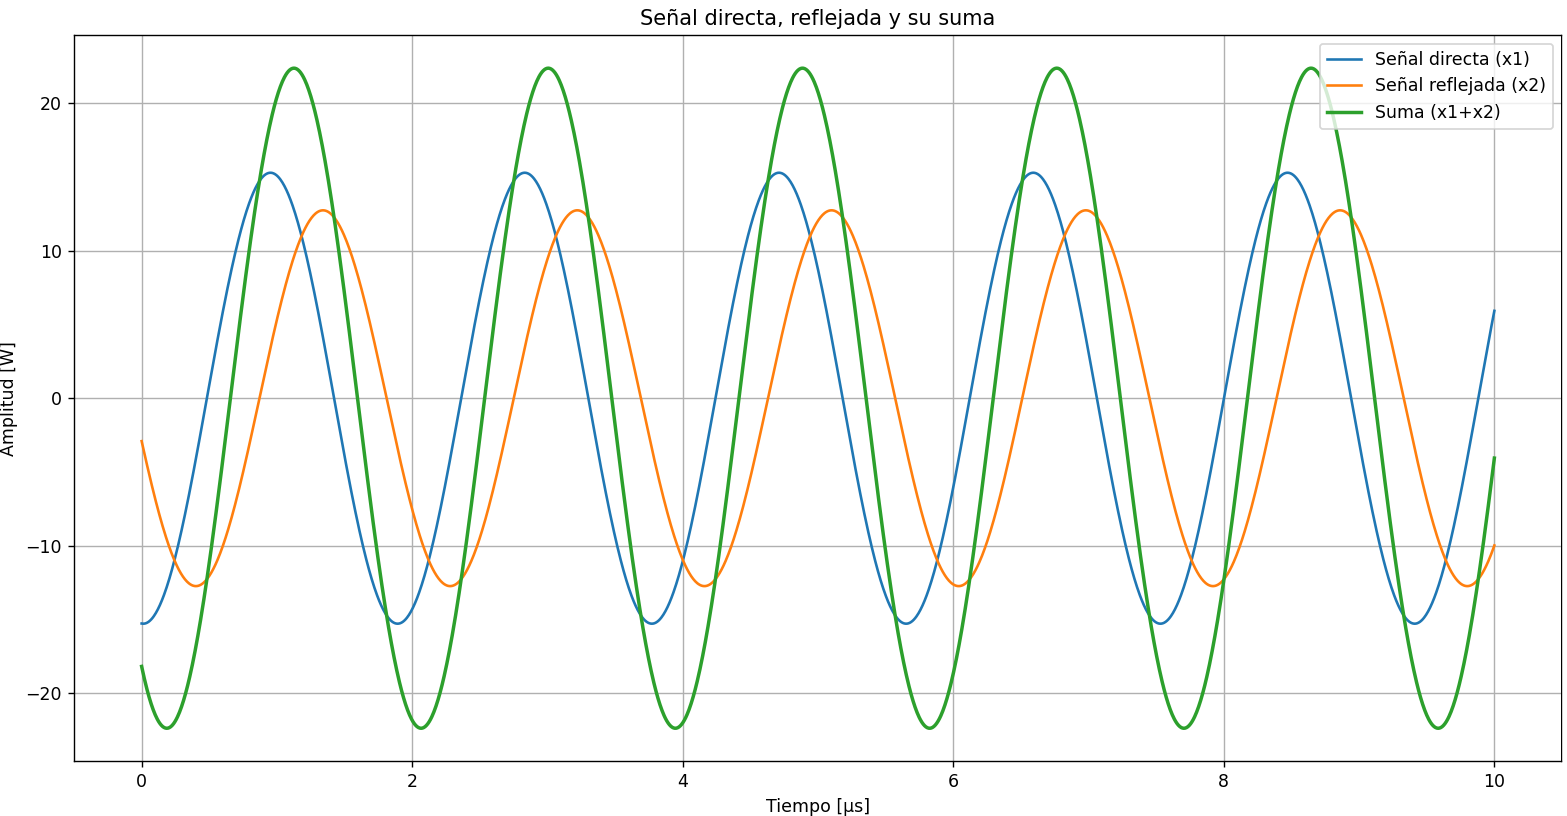
\includegraphics[width=0.8\textwidth]{parte_teorica/grafico_532kHz.png}
\caption{Señal resultante a 532 kHz.}
\end{figure}
\bigskip

En la figura 1 se observa la señal cosenoidal trasmitida en su camino directo y reflejado, la suma de las dos es la que llega a la antena receptora. Como se observa, tienen diferente amplitud y fase debido a las atenuaciones y un retardo temporal por las diferentes distancias.
\bigskip

\noindent \textbf{b) Suponer ahora que la frecuencia aumenta a 600 kHz. ¿Qué sucede? Graficar. }
\bigskip

Hay dos trayectorias:
\[
D_1 = \SI{11}{km} \qquad D_2 = \SI{14.5}{km}.
\]
\bigskip
La diferencia es:
\[
\Delta D = D_2 - D_1 = \SI{3.5}{km} = \SI{3500}{m}.
\]
\bigskip
El retardo entre ambas:
\[
\Delta \tau = \frac{\Delta D}{c} = 
\frac{3500}{3 \cdot 10^{8}}
\approx 1.1667 \times 10^{-5}\,\text{s}.
\]

\bigskip
La diferencia de fase entre ellas es:
\[
\Delta\varphi = 2\pi f \,\Delta\tau.
\]


Las dos señales quedan en fase cuando su diferencia de fase es un múltiplo entero de \(2\pi\):
\[
\Delta\varphi = 2\pi n,\qquad n=0,1,2,\dots
\]


\[
2\pi f \,\Delta\tau = 2\pi n \quad\Longrightarrow\quad f=\frac{n}{\Delta\tau}.
\]
\bigskip
Para \(\Delta\tau=1.1667\times10^{-5}\,\text{s}\):
\[
f_n=\frac{n}{1.1667\times10^{-5}}.
\]
\bigskip
Para \(n=7\):
\[
f_7=\frac{7}{1.1667\times10^{-5}}=600\,\text{kHz}.
\]
\bigskip

A \(f=600\,\text{kHz}\) la diferencia de fase es:
\[
\Delta\varphi=2\pi f \,\Delta\tau=2\pi\cdot 600000\cdot1.1667\times10^{-5}
=2\pi\cdot 7=14\pi,
\]
que es exactamente 7 ciclos completos de diferencia. Por lo tanto, las señales quedan en fase.


\begin{figure}[H]
\centering
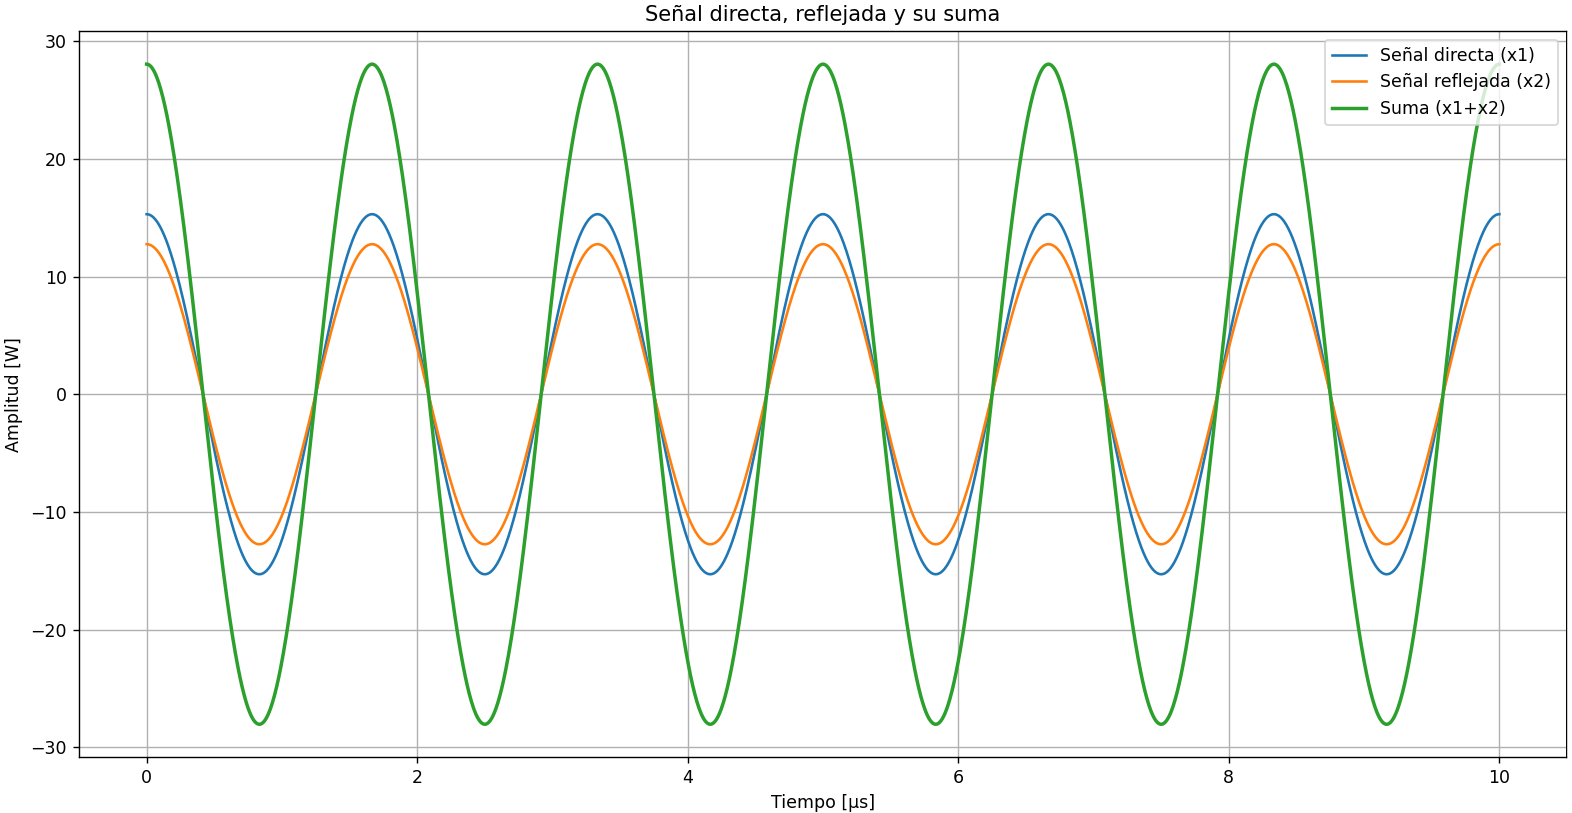
\includegraphics[width=0.8\textwidth]{parte_teorica/grafico_600kHz.png}
\caption{Señal resultante a 600 kHz.}
\end{figure}
 %llama los otros 
    

%\printbibliography[heading=bibintoc] % Agrega el título "Referencias" al índice automáticamente
    
\end{document}